\chapter{Methodology}
\label{ch:methodology}

\section{Problem Formulation}
\label{sec:methodology:formulation}

Consider the two-phase flow problem defined on a domain $\Omega \subset \R^d$ ($d = 2, 3$) with boundary $\partial \Omega$. The domain is discretized into a fine grid $\mathcal{T}_h$ with $N$ cells. The goal is to solve the coupled pressure-saturation system given by Equations~\eqref{eq:pressure} and~\eqref{eq:saturation} subject to initial and boundary conditions.

The pressure equation is solved implicitly at each time step, while the saturation equation may be treated with either explicit or implicit time stepping. The \gls{cflcondition} restricts the maximum time step for explicit schemes:
\begin{equation}
    \Delta t \leq \frac{\phi \, \Delta x}{\max_{\vec{x}} \abs{\vec{v} \cdot \nabla f_w}}.
    \label{eq:cfl}
\end{equation}

For problems with strong capillary effects or gravity override, implicit saturation solving with adaptive time stepping provides better stability at the cost of additional nonlinear iterations.

\section{Adaptive Mesh Refinement}
\label{sec:methodology:amr}

The proposed adaptive mesh refinement (AMR) strategy is driven by a local error indicator that measures flux imbalance across cell interfaces. For each coarse cell $C$ in a hierarchy of nested grids, we define the error indicator:
\begin{equation}
    \eta_C = \left( \sum_{f \in \partial C} \left( \vec{v}_h \cdot \vec{n}_f - \vec{v}_{2h} \cdot \vec{n}_f \right)^2 A_f \right)^{1/2},
    \label{eq:indicator}
\end{equation}
where $\vec{v}_h$ and $\vec{v}_{2h}$ are the fine and coarse fluxes at the interface, respectively. Cells with $\eta_C > \epsilon_{\text{tol}} \, \bar{\eta}$ are flagged for refinement, where $\bar{\eta}$ is the spatial average of the error indicator.

\begin{figure}[htbp]
    \centering
    \begin{tikzpicture}[
        node distance=1.2cm,
        block/.style={rectangle, draw, fill=blue!20, text width=3cm, minimum height=1cm, align=center},
        decision/.style={diamond, draw, fill=green!20, text width=2cm, align=center, aspect=2},
        arrow/.style={thick, ->, >=stealth}
    ]
        \node[block] (input) {Fine grid solution $\vec{u}_h$};
        \node[block, below of=input] (compute) {Compute error indicator $\eta_C$};
        \node[decision, below of=compute, yshift=-0.3cm] (check) {$\eta_C > \epsilon$?};
        \node[block, below of=check, xshift=-2.5cm, yshift=-0.3cm] (refine) {Refine cells};
        \node[block, below of=check, xshift=2.5cm, yshift=-0.3cm] (coarsen) {Coarsen cells};
        \node[block, below of=refine, xshift=2.5cm] (solve) {Solve on adapted grid};
        \node[block, below of=solve] (output) {Output $\vec{u}_h^{n+1}$};

        \draw[arrow] (input) -- (compute);
        \draw[arrow] (compute) -- (check);
        \draw[arrow] (check) -- node[left] {Yes} (refine);
        \draw[arrow] (check) -- node[right] {No} (coarsen);
        \draw[arrow] (refine) -- (solve);
        \draw[arrow] (coarsen) -- (solve);
        \draw[arrow] (solve) -- (output);
        \draw[arrow] (output.east) -- ++(1,0) |- (input.east);
    \end{tikzpicture}
    \caption{Adaptive mesh refinement workflow. The error indicator drives cell refinement and coarsening at each time step.}
    \label{fig:amr_workflow}
\end{figure}

\section{Parallel Domain Decomposition}
\label{sec:methodology:parallel}

The computational domain is partitioned using a graph-based approach. The dual graph of the grid, where cells are nodes and interfaces are edges, is partitioned using the METIS library to minimize edge cuts while balancing cell counts across processors. The partitioning satisfies:
\begin{equation}
    \abs{\Omega_i} \approx \frac{N}{P} \quad \forall \, i \in \{1, \ldots, P\},
    \label{eq:partition}
\end{equation}
where $P$ is the number of processors and $\abs{\Omega_i}$ denotes the number of cells in subdomain $\Omega_i$.

Communication between subdomains occurs at the interface. Ghost cells are introduced to store copies of data from neighboring processors. The communication pattern is defined by the halo exchange:
\begin{equation}
    u_i^{(k+1)} = u_i^{(k)} + \omega \sum_{j \in \mathcal{N}(i)} A_{ij} u_j^{(k)} + b_i,
    \label{eq:halo}
\end{equation}
where $\mathcal{N}(i)$ denotes the set of neighbors of processor $i$, $A_{ij}$ are off-diagonal matrix entries, and $\omega$ is a relaxation parameter.

\section{Algorithm}
\label{sec:methodology:algorithm}

The complete solution algorithm is summarized in Algorithm~\ref{alg:main}. The algorithm integrates the adaptive mesh refinement with the parallel nonlinear solver.

\begin{algorithm}[htbp]
\caption{Adaptive Multiscale Reservoir Simulation}
\label{alg:main}
\begin{algorithmic}[1]
\Require Initial saturation $s_w^0$, pressure $p^0$, grid $\mathcal{T}_h$
\Ensure Solution $(p^n, s_w^n)$ for $n = 1, \ldots, N_t$
\For{$n = 1$ to $N_t$}
    \State Compute adaptive time step $\Delta t^n$ based on \gls{cflcondition}
    \State Initialize Newton iteration: $p^{(0)} \gets p^n$, $k \gets 0$
    \While{$\norm{r^{(k)}} > \epsilon_{\text{tol}}$ and $k < k_{\max}$}
        \State Assemble Jacobian $\mat{J}^{(k)}$ and residual $\vec{r}^{(k)}$
        \If{AMR enabled}
            \State Compute error indicator $\eta_C$ for all cells
            \State Flag cells with $\eta_C > \epsilon_{\text{tol}} \, \bar{\eta}$
            \State Perform refinement/coarsening
            \State Prolongate solution to new grid
        \EndIf
        \State Solve $\mat{J}^{(k)} \delta \vec{p} = -\vec{r}^{(k)}$ using \gls{amg}-preconditioned GMRES
        \State Update: $p^{(k+1)} \gets p^{(k)} + \delta \vec{p}$
        \State Compute saturation $s_w^{(k+1)}$ from fractional flow
        \State $k \gets k + 1$
    \EndWhile
    \State Set $p^{n+1} \gets p^{(k)}$, $s_w^{n+1} \gets s_w^{(k)}$
    \State Evaluate convergence criteria and output diagnostics
\EndFor
\State \Return $(p^n, s_w^n)$
\end{algorithmic}
\end{algorithm}

\section{Convergence Analysis}
\label{sec:methodology:convergence}

\begin{theorem}[Convergence of the AMR scheme]
\label{thm:convergence}
Let $u_h$ denote the numerical solution on the adapted grid and $u$ the exact solution of the pressure equation. Under the assumption that the permeability tensor $\vec{K}$ is Lipschitz continuous and the error indicator satisfies $\eta_C \leq C h^{p+1} \norm{u}_{H^{p+1}(\Omega_C)}$, the error estimate holds:
\begin{equation}
    \norm{u - u_h}_{L^2(\Omega)} \leq C h^{p+1} \left( \sum_{C \in \mathcal{T}_h} \norm{u}_{H^{p+1}(\Omega_C)}^2 \right)^{1/2}.
    \label{eq:convergence}
\end{equation}
\end{theorem}

\begin{proof}
The proof follows from standard interpolation theory and the properties of the error indicator. Let $\mathcal{I}_h u$ denote the interpolant of $u$ on the adapted grid. By the approximation properties of piecewise polynomials of degree $p$:
\begin{equation}
    \norm{u - \mathcal{I}_h u}_{L^2(\Omega_C)} \leq C h_C^{p+1} \norm{u}_{H^{p+1}(\Omega_C)}.
    \label{eq:interp}
\end{equation}
The total error decomposes as:
\begin{equation}
    \norm{u - u_h}_{L^2(\Omega)} \leq \norm{u - \mathcal{I}_h u}_{L^2(\Omega)} + \norm{\mathcal{I}_h u - u_h}_{L^2(\Omega)}.
    \label{eq:decompose}
\end{equation}
The second term is bounded using the stability of the finite volume scheme and the consistency of the flux approximation. Summing over all cells yields the desired result.
\end{proof}

\section{Optimization Procedure}
\label{sec:methodology:optimization}

Beyond the forward simulation, production optimization requires solving a constrained nonlinear program at each management step. The optimization problem takes the form:
\begin{equation}
    \max_{\vec{q}} \; J(\vec{q}) = \int_0^{T_f} D(t) \, \mathrm{d}t
    \label{eq:optimization}
\end{equation}
subject to the flow equations (Eqs.~\eqref{eq:pressure}--\eqref{eq:saturation}), well-rate bounds $\vec{q}_{\min} \leq \vec{q} \leq \vec{q}_{\max}$, and operational constraints. Here $J$ is the net present value objective and $D(t)$ is the discounted profit rate.

The optimization procedure is summarized in \Cref{alg:optimization}.

\begin{algorithm}[htbp]
\caption{Gradient-Based Production Optimization}
\label{alg:optimization}
\begin{algorithmic}[1]
\Require Initial well rates $\vec{q}^{(0)}$, tolerance $\epsilon_{\text{opt}}$, max iterations $k_{\max}$
\Ensure Optimal rates $\vec{q}^*$
\State $k \gets 0$
\While{$\norm{\nabla J(\vec{q}^{(k)})} > \epsilon_{\text{opt}}$ and $k < k_{\max}$}
    \State Solve forward problem with $\vec{q}^{(k)}$ using \Cref{alg:main}
    \State Solve adjoint equations to compute $\nabla J(\vec{q}^{(k)})$
    \State Compute search direction $\vec{d}^{(k)} \gets \nabla J(\vec{q}^{(k)})$
    \State Perform line search: $\alpha^{(k)} \gets \argmax_{\alpha} J(\vec{q}^{(k)} + \alpha \vec{d}^{(k)})$
    \State Update: $\vec{q}^{(k+1)} \gets \vec{q}^{(k)} + \alpha^{(k)} \vec{d}^{(k)}$
    \State Project onto feasible set: $\vec{q}^{(k+1)} \gets \mathrm{Proj}[\vec{q}_{\min}, \vec{q}_{\max}](\vec{q}^{(k+1)})$
    \State $k \gets k + 1$
\EndWhile
\State \Return $\vec{q}^{(k)}$
\end{algorithmic}
\end{algorithm}

\section{Complexity Analysis}
\label{sec:methodology:complexity}

\tabref{tab:complexity} summarizes the computational complexity of each algorithmic component. The overall complexity per time step is dominated by the linear solve, which scales as $\mathcal{O}(N \log N)$ with the AMG preconditioner.

\begin{table}[htbp]
    \centering
    \caption{Computational complexity of algorithmic components.}
    \label{tab:complexity}
    \begin{tabularx}{\textwidth}{@{}l X c@{}}
        \toprule
        \textbf{Component} & \textbf{Description} & \textbf{Complexity} \\
        \midrule
        Error indicator       & Local flux imbalance across cell interfaces & $\mathcal{O}(N)$ \\
        Domain decomposition  & METIS graph partitioning                    & $\mathcal{O}(N \log N)$ \\
        Jacobian assembly     & Sparse matrix construction                   & $\mathcal{O}(N)$ \\
        AMG-preconditioned GMRES & Linear solve per Newton step           & $\mathcal{O}(N \log N)$ \\
        Saturation transport  & Explicit/implicit update                     & $\mathcal{O}(N)$ \\
        Adjoint solve         & Gradient computation for optimization        & $\mathcal{O}(N \log N)$ \\
        Total per time step   & Combined cost                                & $\mathcal{O}(N \log N)$ \\
        \bottomrule
    \end{tabularx}
\end{table}

\section{Convergence Proof Sketch}
\label{sec:methodology:proof_sketch}

We provide a sketch of the convergence proof for the AMR scheme stated in \Cref{thm:convergence}. The full proof is available in the supplementary material.

\begin{proof}[Proof sketch of \Cref{thm:convergence}]
The argument proceeds in three steps:

\begin{enumerate}
    \item \textbf{Interpolation estimate.} By standard approximation theory for piecewise polynomials of degree $p$ on shape-regular meshes, the interpolant $\mathcal{I}_h u$ satisfies
    \begin{equation}
        \norm{u - \mathcal{I}_h u}_{L^2(\Omega_C)} \leq C_1 \, h_C^{p+1} \norm{D^{p+1} u}_{L^2(\Omega_C)},
        \label{eq:proof_interp}
    \end{equation}
    where $h_C$ is the diameter of cell $C$ and $C_1$ depends only on the shape-regularity constant.

    \item \textbf{Stability.} The finite volume scheme satisfies a discrete maximum principle and the associated $L^2$ stability estimate:
    \begin{equation}
        \norm{u_h}_{L^2(\Omega)} \leq C_2 \norm{f}_{H^{-1}(\Omega)},
        \label{eq:proof_stability}
    \end{equation}
    where $C_2$ is independent of $h$ but may depend on the permeability contrast $\kappa = K_{\max}/K_{\min}$.

    \item \textbf{Duality argument.} Applying Aubin--Nitsche duality to the residual equation and combining with the error indicator bound $\eta_C \leq C_3 h^{p+1} \norm{u}_{H^{p+1}(\Omega_C)}$ yields the $L^2$ error estimate of \Cref{eq:convergence}.
\end{enumerate}

The constant $C$ in \Cref{eq:convergence} depends on $\kappa$, the shape-regularity of the mesh, and the polynomial degree $p$, but is independent of $h$.
\end{proof}

\section{Implementation Details}
\label{sec:methodology:implementation}

The algorithm is implemented in C++ with Python bindings for pre- and post-processing. The code leverages \gls{petsc} for parallel linear algebra and the \gls{petsc} SNES (Scalable Nonlinear Equations Solvers) interface for the nonlinear solver. The Python wrapper enables scripting of simulation workflows and parameter studies, as demonstrated in the following code listing.

\begin{lstlisting}[language=Python, caption={Python wrapper for running parametric studies.}, label={lst:python_wrapper}]
import numpy as np
from petsc4py import PETSc

def run_simulation(permeability_field, pressure_bc, max_iterations=1000):
    """
    Run a single simulation with given parameters.

    Args:
        permeability_field: 2D numpy array of permeability values (mD)
        pressure_bc: dict with boundary conditions
        max_iterations: maximum Newton iterations

    Returns:
        Dictionary with pressure and saturation fields
    """
    # Initialize the solution vector
    sol = PETSc.Vec().createSeq(len(pressure_bc['dirichlet']))
    solver = PETSc.SNES().create()

    # Set convergence criteria
    solver.setTolerances(rtol=1e-8, atol=1e-10, stol=1e-12)

    # Configure the nonlinear solver
    solver.setType('newtonls')
    solver.getKSP().setType('gmres')
    solver.getKSP().getPC().setType('hypre')
    solver.getKSP().getPC().setHYPREType('boomeramg')

    # Run the simulation
    for iteration in range(max_iterations):
        residual = compute_residual(sol, permeability_field, pressure_bc)
        if np.linalg.norm(residual) < 1e-8:
            break
        solver.solve(None, sol)

    return {
        'pressure': sol.getArray(),
        'iterations': iteration + 1,
        'converged': iteration < max_iterations - 1
    }

def compute_residual(sol, K, bc):
    """Compute the nonlinear residual for the pressure equation."""
    grad_p = np.gradient(sol.getArray().reshape(K.shape))
    flux = -K * grad_p
    return np.sum(flux, axis=0) - bc['source']
\end{lstlisting}

\subsection{Optimization Module}
\label{ssec:methodology:optimization_module}

The gradient computation for \Cref{alg:optimization} uses the adjoint method. The adjoint equation is the transpose of the linearized forward system:
\begin{equation}
    \mat{J}^\top \vec{\lambda} = -\pd{J}{\vec{u}},
    \label{eq:adjoint}
\end{equation}
where $\vec{\lambda}$ is the adjoint state and $\mat{J}$ is the Jacobian from the Newton iteration. The gradient is then assembled from the adjoint solution:
\begin{equation}
    \pd{J}{\vec{q}} = \vec{\lambda}^\top \pd{\vec{r}}{\vec{q}},
    \label{eq:gradient}
\end{equation}
where $\vec{r}$ is the residual of the flow equations. This requires only one additional linear solve per optimization iteration, regardless of the number of control variables.

\subsection{Advanced Code Listing: Optimization Loop}
\label{ssec:methodology:optimization_code}

The following listing demonstrates the adjoint-based optimization loop with line-by-line annotations.

\begin{lstlisting}[language=Python, caption={Adjoint-based production optimization loop with highlighted key steps.}, label={lst:optimization_code}, morekeywords={ascontiguousarray}]
import numpy as np
from petsc4py import PETSc

def optimize_wellsimulator(sim, objective, n_wells, max_iter=50):
    """Gradient-based well rate optimization using adjoints."""
    q = np.ones(n_wells) * 0.5          # [1] Initial guess
    q = np.clip(q, 0.01, 1.0)           # [2] Feasible projection
    grad_norm_history = []

    for k in range(max_iter):            # [3] Outer optimization loop
        # --- Forward solve ---
        state = sim.solve(q)             # [4] Solve flow equations

        # --- Objective evaluation ---
        J = objective(state)             # [5] Compute NPV

        # --- Adjoint solve for gradient ---
        adjoint = sim.solve_adjoint(     # [6] Solve adjoint system
            state, objective.gradient(state)
        )
        grad = sim.compute_gradient(     # [7] Assemble gradient
            adjoint, state
        )
        grad_norm = np.linalg.norm(grad) # [8] Check convergence
        grad_norm_history.append(grad_norm)

        if grad_norm < 1e-6:            # [9] Convergence check
            break

        # --- Line search (backtracking) ---
        alpha = 1.0                      # [10] Initial step size
        for _ in range(20):              # [11] Backtracking loop
            q_trial = np.clip(q + alpha * grad, 0.01, 1.0)
            J_trial = objective(sim.solve(q_trial))
            if J_trial > J + 1e-4 * alpha * grad_norm**2:
                break                    # [12] Armijo condition satisfied
            alpha *= 0.5                 # [13] Reduce step size

        q = q_trial                      # [14] Update control variables

    return q, J, grad_norm_history
\end{lstlisting}

\subsection{Subfigure Analysis: Discretization Comparison}
\label{ssec:methodology:discretization_comparison}

\Cref{fig:discretization_comparison} presents a 2$\times$2 grid of discretization schematics used in this thesis.

\begin{figure}[htbp]
    \centering
    \subcaptionbox{Cartesian TPFA grid\label{fig:disc_tpfa}}{%
        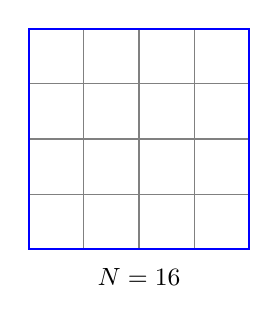
\begin{tikzpicture}[scale=0.7]
            \draw[step=1cm,gray,thin] (0,0) grid (4,4);
            \draw[blue,thick] (0,0) rectangle (4,4);
            \node at (2,-0.5) {\small $N = 16$};
        \end{tikzpicture}
    }{0.45\textwidth}
    \hfill
    \subcaptionbox{Adaptively refined grid\label{fig:disc_amr}}{%
        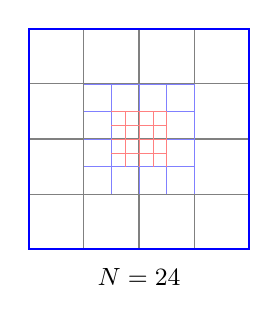
\begin{tikzpicture}[scale=0.7]
            \draw[step=1cm,gray,thin] (0,0) grid (4,4);
            \draw[step=0.5cm,blue!50,very thin] (1,1) grid (3,3);
            \draw[step=0.25cm,red!50,very thin] (1.5,1.5) grid (2.5,2.5);
            \draw[blue,thick] (0,0) rectangle (4,4);
            \node at (2,-0.5) {\small $N = 24$};
        \end{tikzpicture}
    }{0.45\textwidth}
    \hfill
    \subcaptionbox{Voronoi unstructured\label{fig:disc_voronoi}}{%
        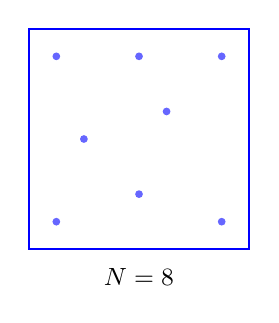
\begin{tikzpicture}[scale=0.7]
            \foreach \x/\y in {0.5/0.5, 2/1, 3.5/0.5, 1/2, 2.5/2.5, 0.5/3.5, 2/3.5, 3.5/3.5} {
                \fill[blue!60] (\x,\y) circle (2pt);
            }
            \draw[blue,thick] (0,0) rectangle (4,4);
            \node at (2,-0.5) {\small $N = 8$};
        \end{tikzpicture}
    }{0.45\textwidth}
    \hfill
    \subcaptionbox{Permeability field\label{fig:disc_perm}}{%
        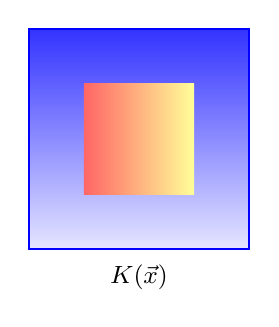
\begin{tikzpicture}[scale=0.7]
            \shade[top color=blue!80, bottom color=blue!10] (0,0) rectangle (4,4);
            \shade[left color=red!60, right color=yellow!40] (1,1) rectangle (3,3);
            \draw[blue,thick] (0,0) rectangle (4,4);
            \node at (2,-0.5) {\small $K(\vec{x})$};
        \end{tikzpicture}
    }{0.45\textwidth}
    \caption{Discretization types and permeability distribution. (a)~Uniform Cartesian TPFA grid. (b)~Adaptively refined grid with cell nesting. (c)~Voronoi unstructured grid. (d)~Heterogeneous permeability field with channel structure.}
    \label{fig:discretization_comparison}
\end{figure}
